% 五号字体,开明式标点处理,不设置默认字体
\documentclass[UTF8, 12pt, punct=kaiming, fontset=none]{article}
\usepackage[UTF8]{ctex}
\usepackage{fontspec}
\usepackage{float}
\usepackage{graphicx}
\usepackage{subcaption}
\usepackage{pgf-umlsd}
% 品红色链接和注释
% \usepackage[colorlinks=true, linkcolor=magenta, citecolor=magenta, urlcolor=magenta]{hyperref}
% 黑色链接和注释
\usepackage[colorlinks=true, linkcolor=black, citecolor=black, urlcolor=black]{hyperref}
\usepackage{geometry}
\usepackage{fancyhdr}
\usepackage{caption}
\usepackage{framed}
\usepackage{titlesec}
\usepackage{ragged2e}
\usepackage{url}
\usepackage{cite}
\usepackage{bookmark}

\graphicspath{{figures/}}

% 字体
\IfFontExistsTF{Source Han Serif SC}
{
    \setCJKmainfont{Source Han Serif SC}
}
{
    % GitHub Actions
    \setCJKmainfont[
        Path=. ./fonts/ ,    
        Extension = . otf ,
        UprightFont = *-Regular ,
        BoldFont = *-Bold
    ]{SourceHanSerifSC}
}
\IfFontExistsTF{Source Han Sans SC}
{
    \setCJKsansfont{Source Han Sans SC}
}
{
    % GitHub Actions
    \setCJKsansfont[
        Path=. ./fonts/ ,    
        Extension = . otf ,
        UprightFont = *-Regular ,
        BoldFont = *-Bold
    ]{SourceHanSerifSC}
}
\IfFontExistsTF{DejaVu Sans}
{
    \newfontfamily\ds{DejaVu Sans}
}
{
    % GitHub Actions
    \newfontfamily\ds[
        Path=. ./fonts/ ,    
        Extension = . ttf ,
        BoldFont = *-Bold ,
        ItalicFont = *-Oblique ,
        BoldItalicFont = *-BoldOblique
    ]{DejaVuSans}
}
%\newfontfamily\cm{CMU}

% 图表标题字体
\DeclareCaptionFont{captionfont}{\ds}
\captionsetup[table]{font=captionfont}
\captionsetup[figure]{font=captionfont}


% 布局
\geometry{a4paper, left=2cm, right=2cm, top=2.5cm, bottom=2.5cm}
\setlength{\headheight}{25pt}

% 页眉页脚
\pagenumbering{arabic}
\pagestyle{fancy}
\fancyhead[L]{\ds · \hspace{0.1cm} \thepage \hspace{0.1cm} ·}
\fancyhead[C]{\ds 红~石~数~电~评~论\\\scriptsize{Review of Redstonic Digital Circuit}}
\fancyhead[R]{\ds 第1期\\\scriptsize{2022年1月}}
\fancyfoot[L, C, R]{}

% 标题
\title{\vspace{-1.5cm}串行二进制转十进制方案\vspace{-0.5cm}}
\author{@天启c}
\date{}

% 参考文献标注
\newcommand*{\upcite}[1]{
    \textsuperscript{\cite{#1}}
}

\begin{document}
    \maketitle
    \thispagestyle{fancy} % 首页页眉页脚
    \vspace{-0.7cm}

    % 节标题格式
    \titleformat{\section}[hang]{\large\sffamily\bfseries}{\textmd{\ds\thesection}}{0.5cm}{}
    \titlespacing{\section}{0cm}{0.5ex}{0.2ex}
    \setcounter{section}{-1}

    数据在计算机中是二进制的形式存在的,十进制的数字同样也是用二进制数的形式存储。在计算机中通常有将十进制(BCD)码转换为二进制(BIN)码,又将二进制码转换为十进制码的操作。我们完全可以在Minecraft中将该操作进行还原。本文提出的“二转十”机器使用串行“满五加三”算法 \cite{5_3},以数据流移位器为核心,利用查表法执行算法,配合时钟和RS锁存器,可以每6tick计算一个二进制位。

    串行信号首先发送到BIN码区,并不断向高位移位。超过8位的数据进入BCD码区。BCD码每四位一组依次代表十进制的某一位的值。在BIN码向BCD码移位操作过程中,我们通过“满五加三”算法完成由BIN码到BCD码的转换。这里我们通过查表法实现该算法。
    
\begin{figure}[!hb]
    \centering
    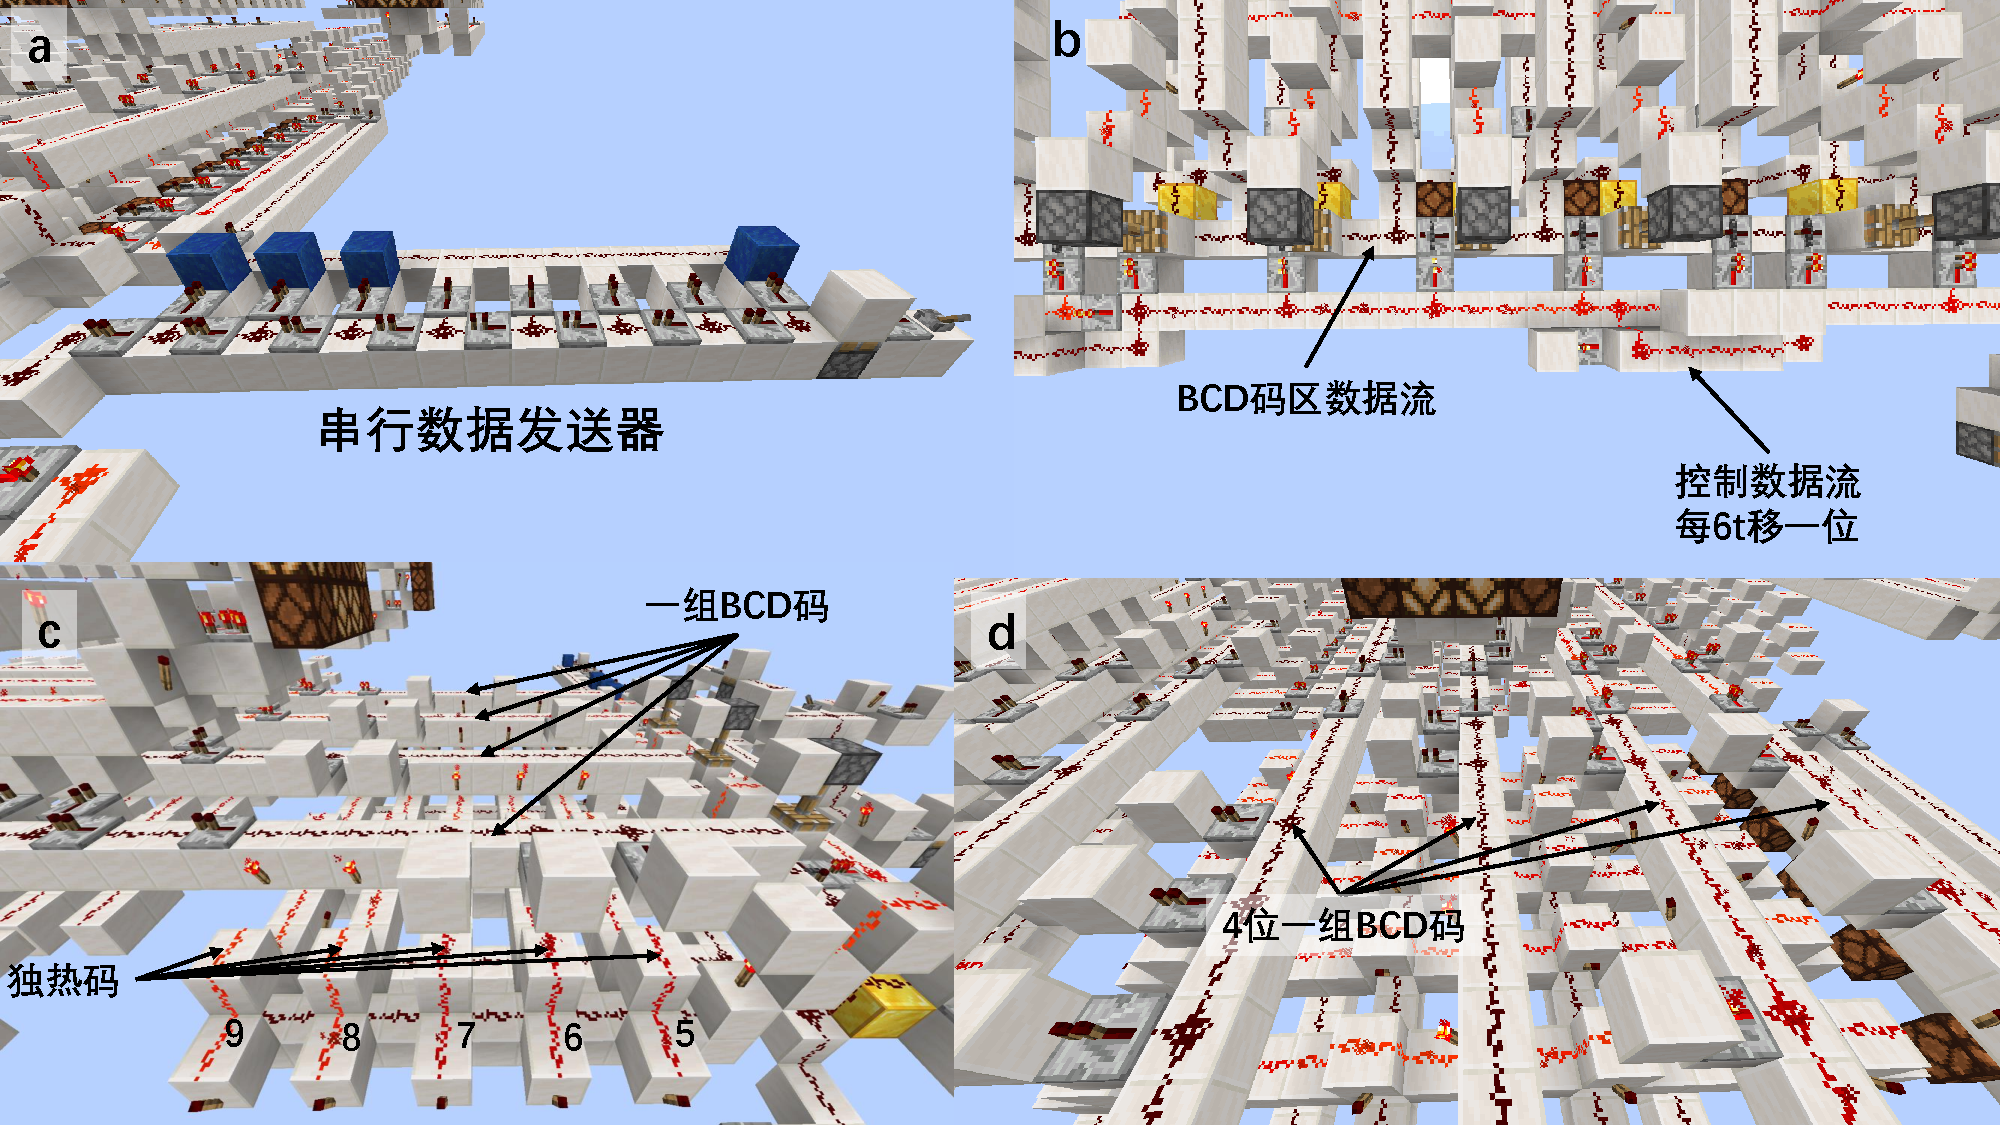
\includegraphics[width=.9\textwidth]{Fig_1.pdf}
    \caption{(a)(b) 串行数据发送器将数据流发送到移位器。(c)(d) 每一组BCD码信号按行输入,逐列比较。对于每一列独热码,红石火把代表1,红石中继器石英块代表0。当且仅当数值与某列信号匹配时,下方红石信号线(独热码线)熄灭,其上的红石火把点亮(独热码输出)。独热码会重新编码“加三”后的结果,并输出到(b)中金块的位置。}
    \label{fig:1}
\end{figure}

查表包含两个步骤。首先是寻址:将多个端口用二进制编码,并用二进制地址来激发相应端口。如果输入的是5,6,7,8,9(即满五),则寻址器会激发对应的独热码,见图\ref{fig:1}(c)(d)。接下来,被激发的独热码会通过解码器向数据流移位器反馈“加三”后的结果,即8,9,10,11,12,并替换该组BCD码。如果输入不满五,则不做动作。修改完毕后,BIN码和BCD码都向高位移动一位。重复这一流程直到BIN码区清空,则BCD码区就是输入转换成十进制的结果。

\begin{figure}[t]
    \centering
    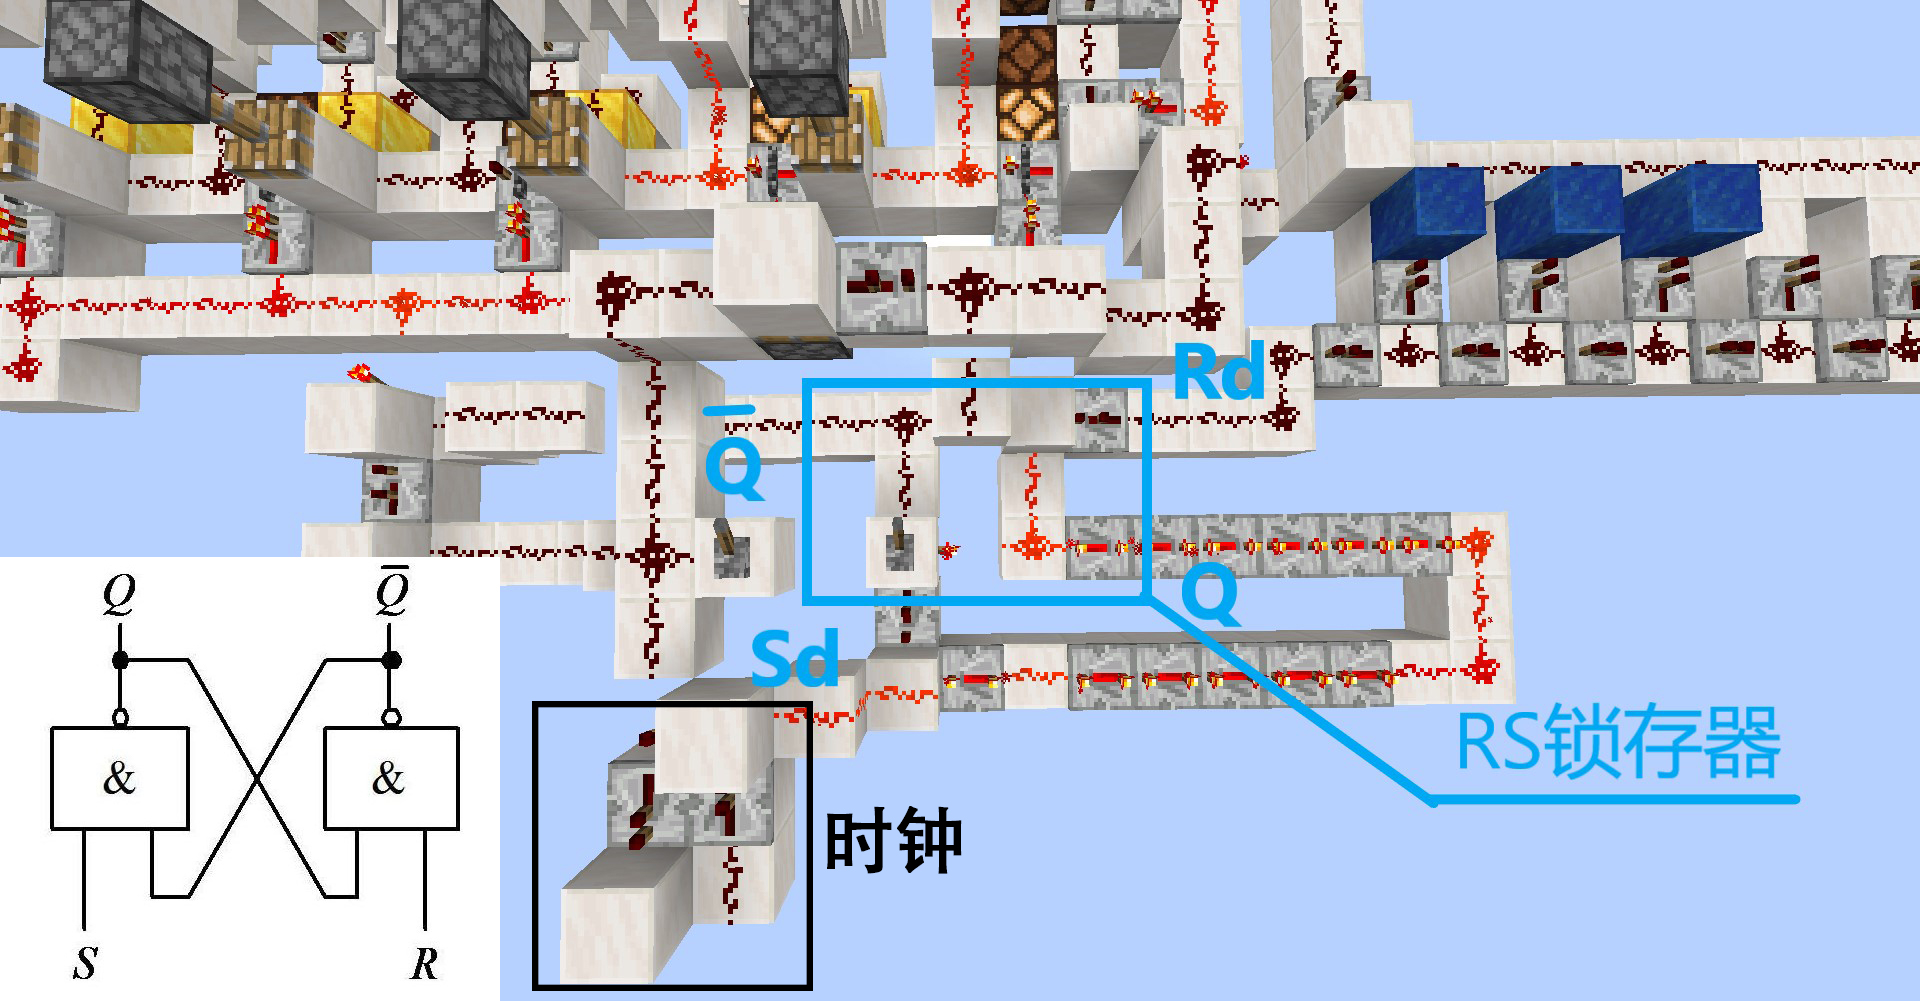
\includegraphics[width=.9\textwidth]{Fig_2.jpg}
    \caption{控制电路。开始信号以脉冲形式输入Rd并将RS锁存器置1,随后中继器链陆续熄灭,并在48tick后将RS锁存器清零。在RS锁存器置1期间,时钟启动并为机器提供6tick周期的脉冲信号。时钟输出的3tick脉冲会被调整为2tick,以此控制移位器每次移一位。左下角为RS锁存器逻辑电路。}
    \label{fig:2}
\end{figure}

控制组件包括一个周期为6tick的时钟,RS锁存器和一组48tick中继器延时,其目的是为机器提供8个时钟脉冲信号,见图\ref{fig:2}。不同的转换位数和布线方案会导致具体中继器延时与48tick有出入,需按具体情况作更改。

本文提出的串行“二转十”方案较并行方案体积小很多,而且很容易拓展,可以运用在四则计算器等需要显示十进制结果的机器上。为Minecraft数电红石技术发展新的计算器结构提供了新的研究方向。

\bibliographystyle{unsrt}
\bibliography{reference.bib}

\end{document}

